\chapter{Experiments, Results and Implementation}
\label{chapter:ch4}

In this chapter the process and results of multiple experiments, that look into performance of various pre-trained feature extractors in industrial anomaly detection tasks, will be presented. First experiment serves to determine the layers of vision transformer architecture that would provide the highest accuracy for anomaly detection when applied as backbones. Secondly, the analysis on the efficacy of self-supervised model DINO against supervised classification task training, helping us to make the decision for verifying the method for feature learning. Next, we will provide a performance comparison between different types of deep learning visual models as feature extractors on the PatchCore model, in order to determine which architecture should be chosen for further experiments. Further, we test the feature space learned from the dataset constructed by the method of selective extraction using CNN bi-class classifiers. Generated feature space competes against one of the state-of-the-art feature spaces for industrial anomaly detection: WideResNet50. Lastly, we will engage in a comparative analysis of the efficiency of the feature space based on a dataset extracted through a method that employs both large language models (LLMs) and visual language models (VLMs). Through these comprehensive experiments and analyses, we aim to derive valuable insights and optimal approaches for advancing industrial anomaly detection by approaching the task as a feature space problem.

\section{Scoring methodology}

\subsection{Scoring metric}
For all the experiments, in order to measure the accuracy of the models being tested, we use AUROC (Area Under the Receiver Operating Characteristic curve) metric. AUROC metric represent the models capability to determine true positives while keeping the number of false positives relatively low. ROC curve, as shown in the figure \ref{fig:auroc}, is the curve that represents the relationship between TPR and FPR at any given threshold. TPR and FPR at an arbitrary threshold is calculated by equations \ref{eq:tpr} and \ref{eq:fpr} respectively. AUROC score is represented as a number between 0 and 1.0(higher the better) and generally, the score 0.5 represents the random guessing. Therefore, scores below 0.5 are considered worse than random guessing while above 0.5 are better. Figures in this paper represent the AUROC score as the percentage from 0\% to 100\%.

\begin{equation}
	TPR = \frac{\text{True Positives}}{\text{True Positives} + \text{False Negatives}}
	\label{eq:tpr}
\end{equation}

\begin{equation}
	FPR = \frac{\text{False Positives}}{\text{False Positives} + \text{True Negatives}}
	\label{eq:fpr}
\end{equation}

\begin{figure}[h]
	\begin{center}
		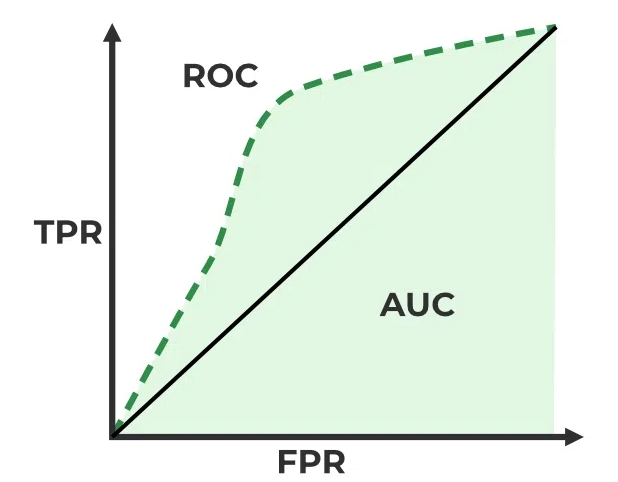
\includegraphics[width=0.5\linewidth]{Chapter_4/auroc.png}
	\end{center}
	\caption{AUROC score is a area under ROC curve represented as a relationship of TPR and FPR.}
	\label{fig:auroc}
\end{figure}

\subsection{Industrial Anomaly detection model}
The model of choice for all the tests is the PatchCore model, as it allows an easy plug and play approach to pre-trained feature extractors. PatchCore outputs three types of scores for each category in the MVTechAd dataset. There are also mean scores over all cotegories provide for each type of scores. Types of scores are as follows:

\begin{description}
  \item[Instance AUROC] represents AUROC score for classifying each image as anomalous or nominal
  \item[Anomaly Pixel AUROC] represents AUROC score for classifying each pixel as anomalous or nominal, calculated only on images that contain anomalies
  \item[Full Pixel AUROC] represents AUROC score for classifying each pixel as anomalous or nominal, calculated over all images
\end{description}

In order to be able to utilize Vision Transformer architectures with PatchCore model, the following changes have been made. These changes detect if the ViT is being used as pre-trained feature extractor and reshape the layers as appropriate for PatchCore.

\lstset{frame=tb,
  language=Python,
  aboveskip=3mm,
  belowskip=3mm,
  showstringspaces=false,
  columns=flexible,
  basicstyle={\small\ttfamily},
  numbers=none,
  numberstyle=\tiny\color{gray},
  breaklines=true,
  breakatwhitespace=true,
  tabsize=3
}
\begin{lstlisting}
def patchify(self, features, return_spatial_info=False):
	#...
	if len(features.shape) == 3:
		features = features.transpose(1, 2)
		if features.shape[2] == 197:
			features = features[:, :, 1:]
		hw = int(math.sqrt(features.shape[2]))
		features = features.view(features.shape[0], features.shape[1], hw, hw)
	#...
\end{lstlisting}

\section{Comparison of ViT layers}
\label{vit layers}

In the first experiment we will be analysing the difference of the layers of vision transformer architectures. Throughout the experiment we use VitB/16 pre-trained on ImageNet classification task. PatchCore research paper recommend using the features from one layer, or aggregating features from up to two layers in order to achieve best results. The results in the figure \ref{fig:vit_layers} indicate Instance AUROC mean scores across all the categories in the dataset MVTechAd. As displayed in the figure \ref{fig:vit_layers}, the best approach is the utilization of the layer 8 alone. This approach achieves the highest score of 94.38\%. For all the experiments involving Vision Transformer architecture, we will be opting for layer 8 of VitB/16 model.

\begin{figure}[h]
	\begin{center}
		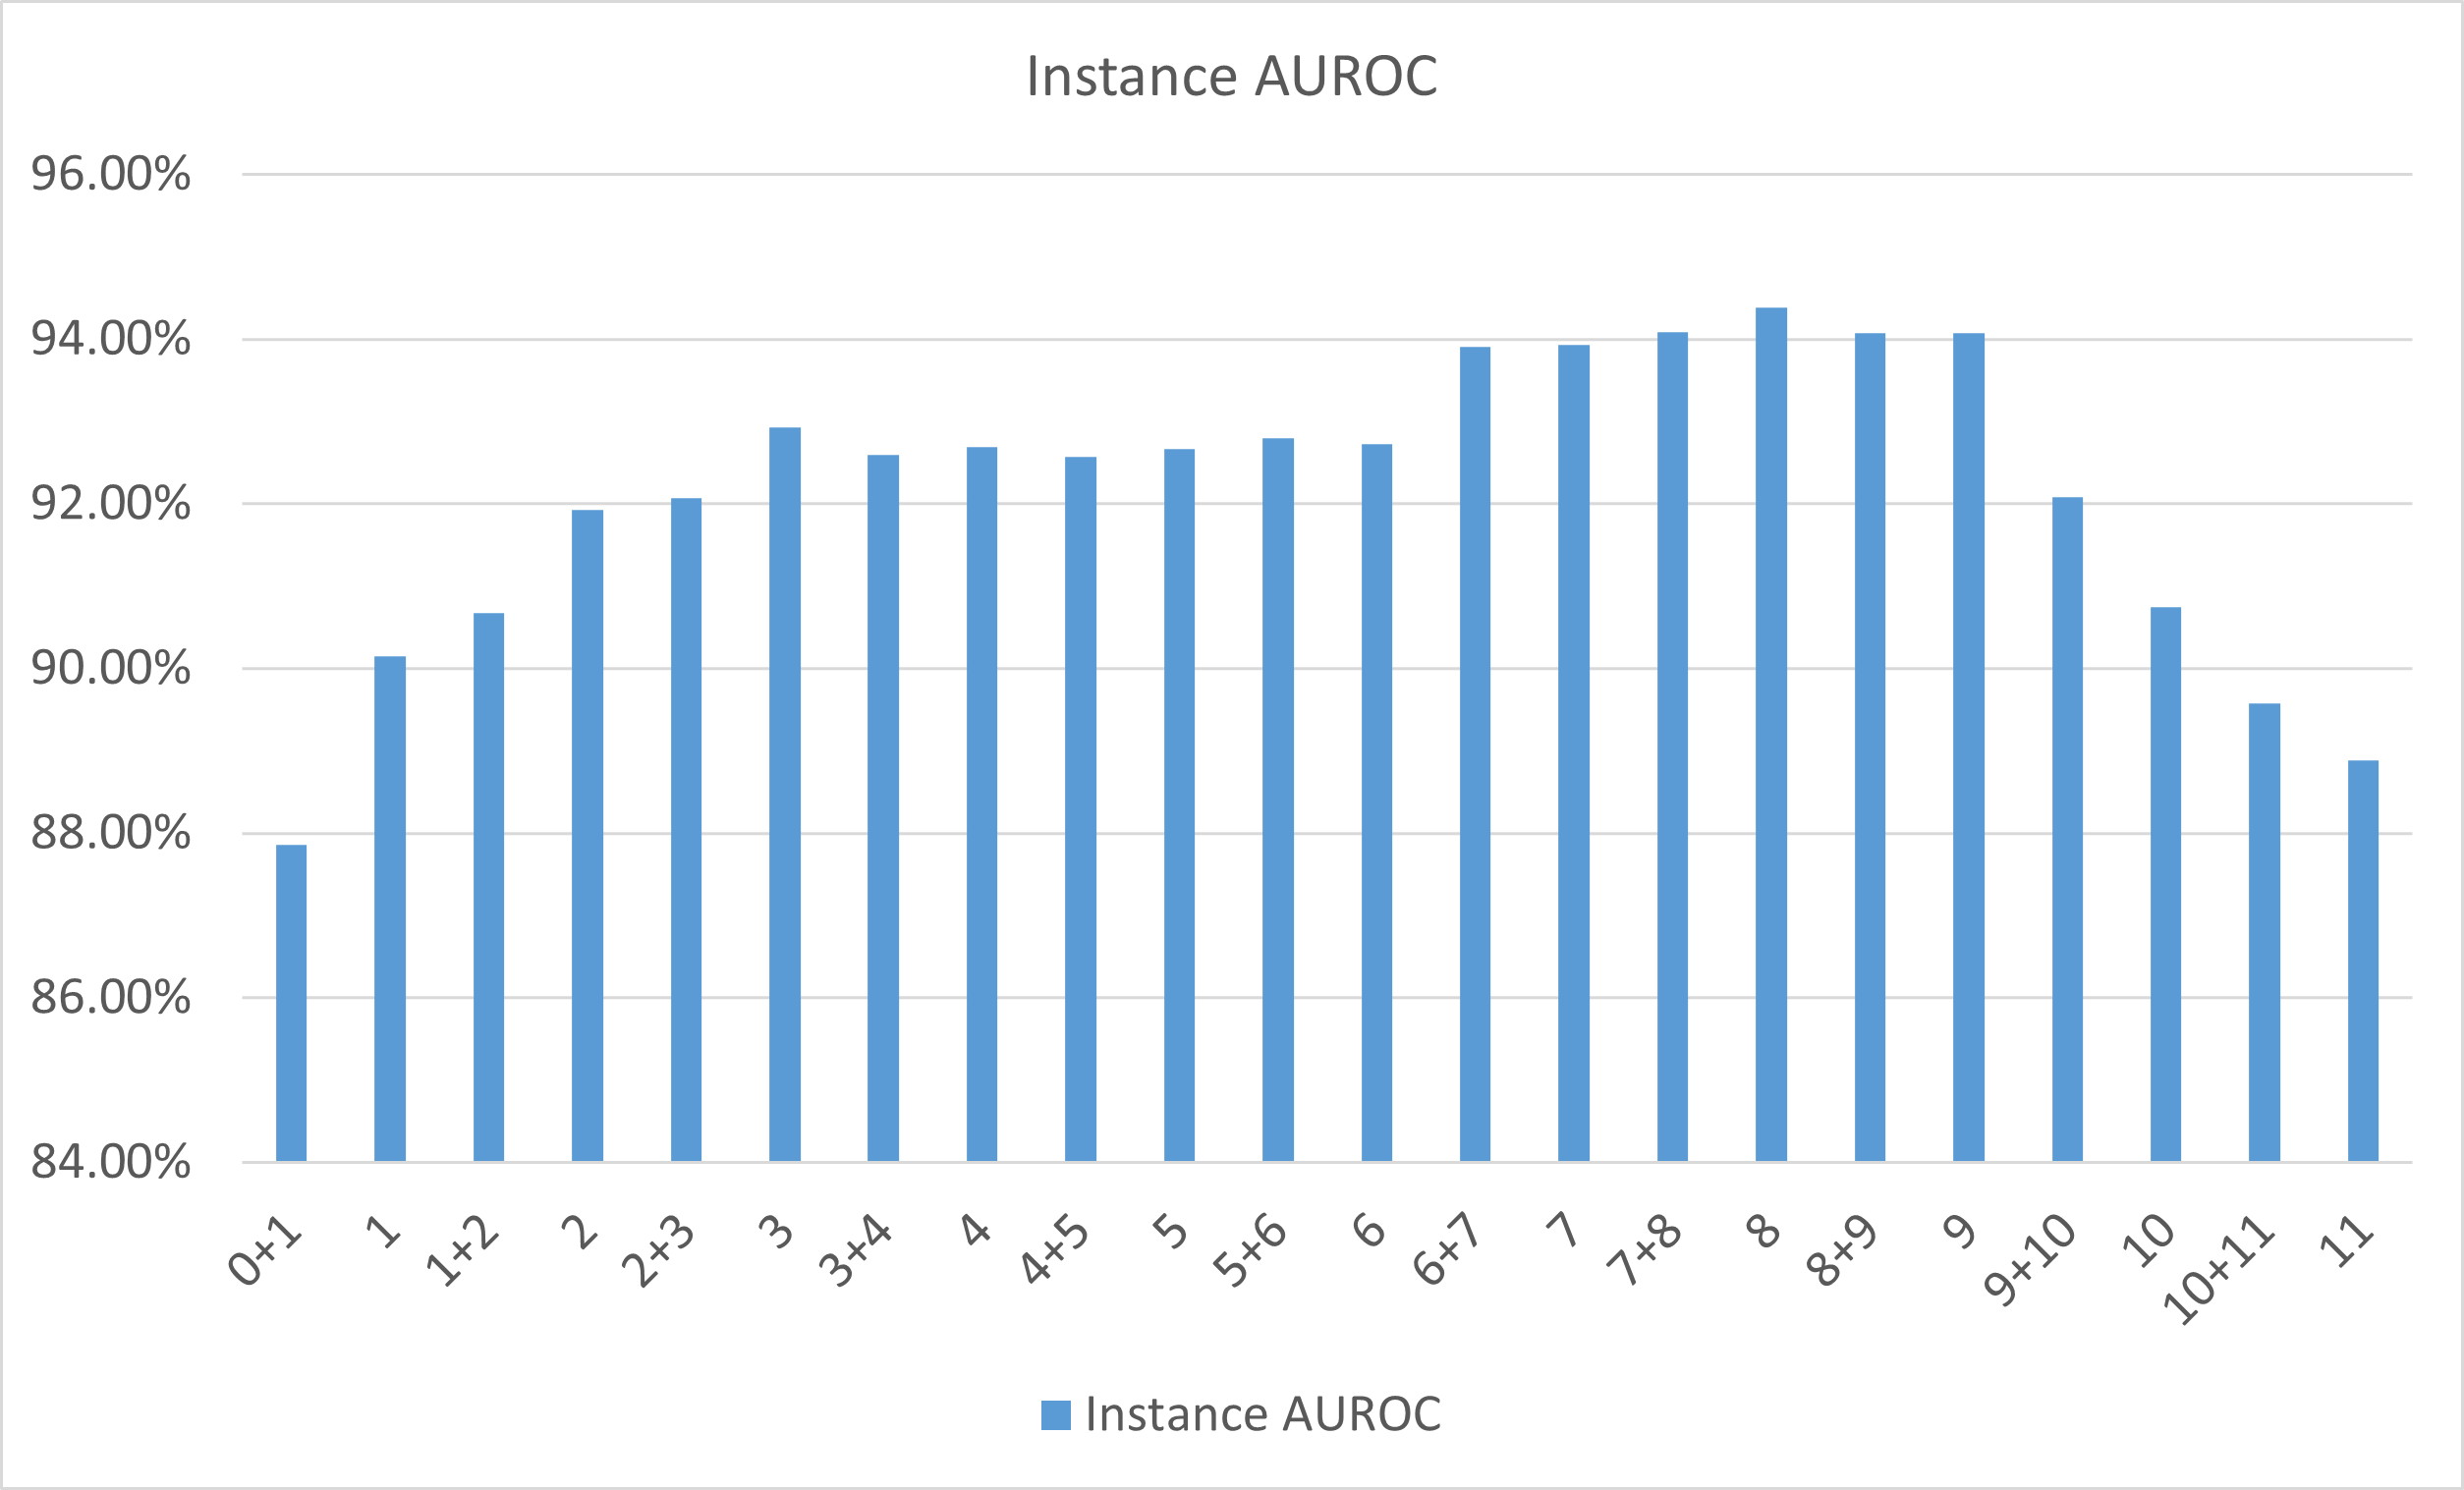
\includegraphics[width=1.0\linewidth]{Chapter_4/vit.png}
	\end{center}
	\caption{Mean Instance AUROC score across all categories of MVTechAd for PatchCore with VitB/16 pre-trained extractor.}
	\label{fig:vit_layers}
\end{figure}

\section{Superiority of WideResNet50 over ResNet50}
In the following experiment we show that WideResNet50 architecture has an overhead of efficiency against ResNet50 architecture. Analysing the figure \ref{fig:resnet_vs_wideresnet} we can clearly see that WideResNet50 has better performances in all the mean scores. Following this discovery, and the conclusion from the next experiment, we opt for the usage of WideResNet50 model to learn features from extracted datasets.

\begin{figure}[h]
	\begin{center}
		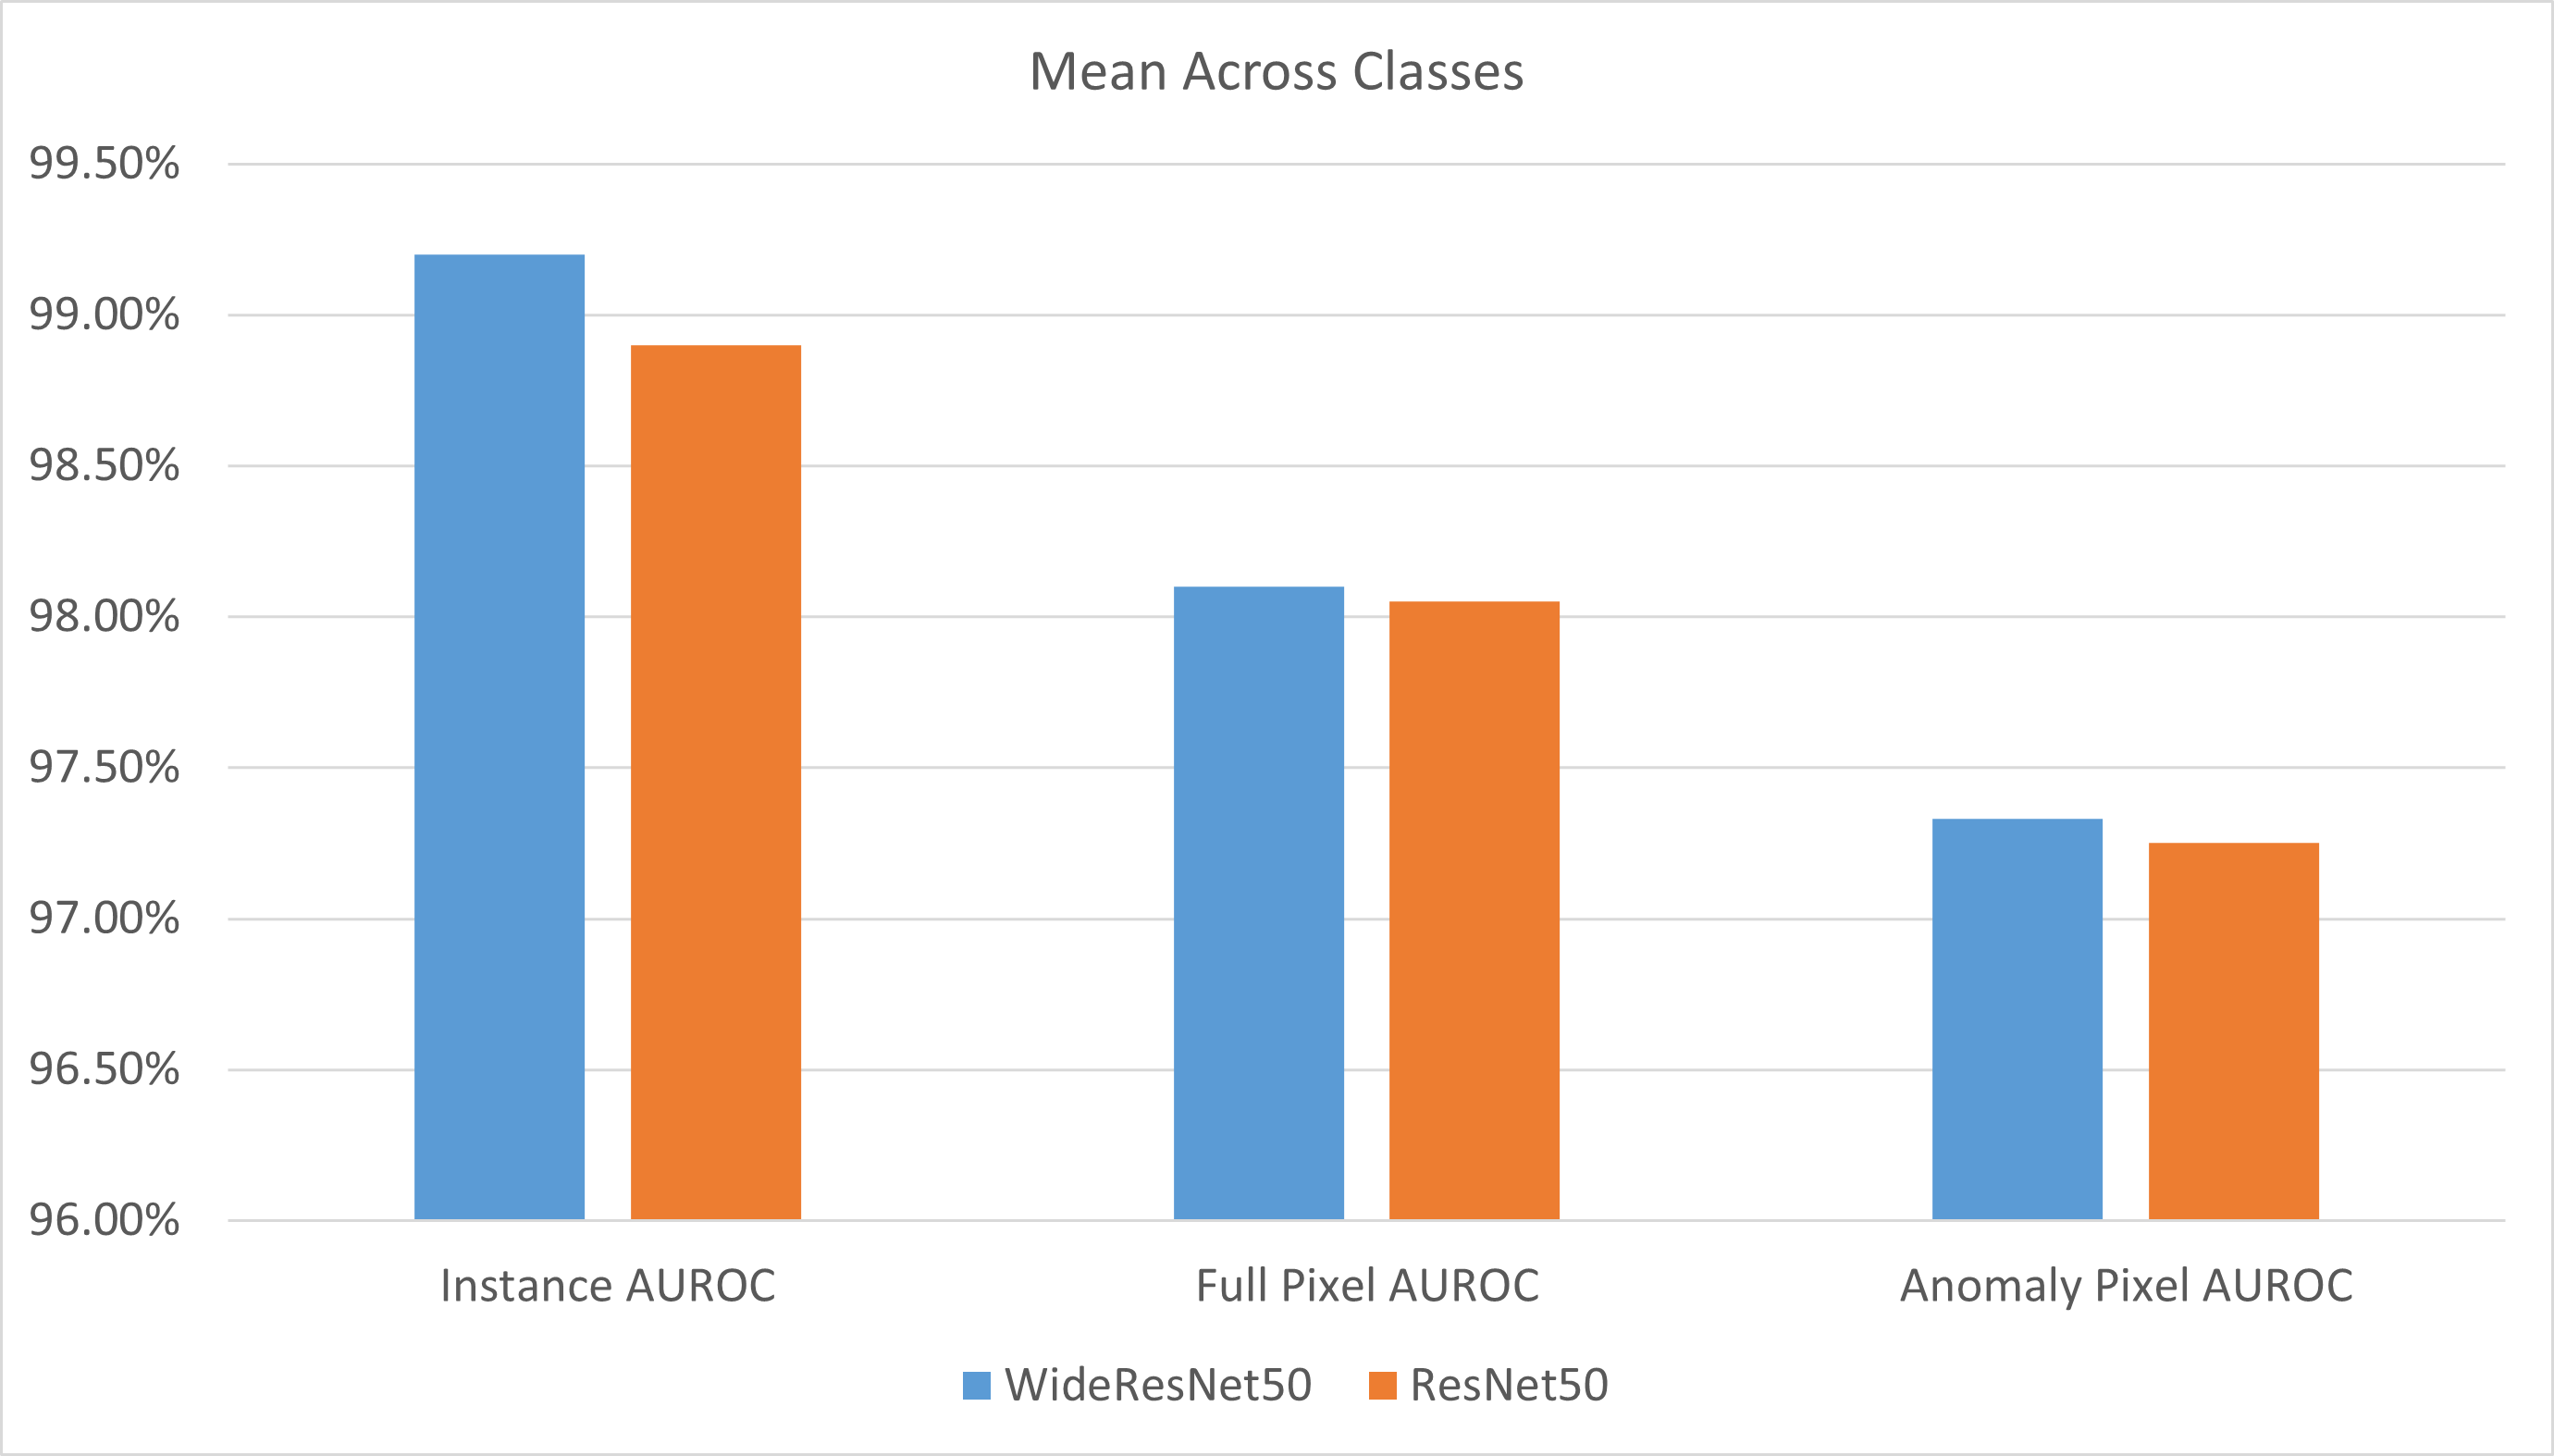
\includegraphics[width=1.0\linewidth]{Chapter_4/resnet_vs_wideresnet.png}
	\end{center}
	\caption{Mean Instance AUROC, Full Pixel AUROC and Anomaly AUROC scores of different layers of VitB/16 model across all categories.}
	\label{fig:resnet_vs_wideresnet}
\end{figure}

\section{Analysis on the efficieny of DINO model}
\label{sec:dino_tests}
In this experiment we aim to determine if the self-supervised training model is capable enough to compete with the supervised learning methods in generating feature spaces for the use in IAD models. We compare ResNet50 model the pre-trained using supervised classification method by the PyTorch team and ResNet50 pre-trained using DINO self-supervised learning mode. Both models are trained on ImageNet1K dataset. Below we provide recipes for training each model.

PyTorch pre-trained ResNet50:

\lstset{frame=tb,
  language=bash,
  aboveskip=3mm,
  belowskip=3mm,
  showstringspaces=false,
  columns=flexible,
  basicstyle={\small\ttfamily},
  numbers=none,
  numberstyle=\tiny\color{gray},
  breaklines=true,
  breakatwhitespace=true,
  tabsize=3
}
\begin{lstlisting}
torchrun --nproc_per_node=8 train.py --model $MODEL_NAME --batch-size 128 \ 
--lr 0.5 --lr-scheduler cosineannealinglr --lr-warmup-epochs 5 \
--lr-warmup-method linear --auto-augment ta_wide --epochs 600 \ 
--random-erase 0.1 --weight-decay 0.00002 --norm-weight-decay 0.0 \ 
--label-smoothing 0.1 --mixup-alpha 0.2 --cutmix-alpha 1.0 \
--train-crop-size 176 --model-ema --val-resize-size 232
\end{lstlisting}

DINO pre-trained ResNet50:

\lstset{frame=tb,
  language=json,
  aboveskip=3mm,
  belowskip=3mm,
  showstringspaces=false,
  columns=flexible,
  basicstyle={\small\ttfamily},
  numbers=none,
  numberstyle=\tiny\color{gray},
  breaklines=true,
  breakatwhitespace=true,
  tabsize=3
}
\begin{lstlisting}
{
	"arch": "resnet50", 
	"out_dim": 60000, 
	"norm_last_layer": true, 
	"warmup_teacher_temp": 0.04, 
	"teacher_temp": 0.07, 
	"warmup_teacher_temp_epochs": 50, 
	"use_fp16": false, 
	"weight_decay": 0.000001, 
	"weight_decay_end": 0.000001, 
	"clip_grad": 0, 
	"batch_size_per_gpu": 51, 
	"epochs": 800, 
	"freeze_last_layer": 1, 
	"lr": 0.3, 
	"warmup_epochs": 10, 
	"min_lr": 0.0048, 
	"global_crops_scale": [0.14, 1.0], 
	"local_crops_scale": [0.05, 0.14], 
	"local_crops_number": 6, 
	"seed": 0, 
	"num_workers": 10, 
	"world_size": 80, 
	"optimizer": "lars", 
	"momentum_teacher": 0.996, 
	"use_bn_in_head": true
}
\end{lstlisting}

The figure \ref{fig:dino_test} shows the mean scores Instance AUROC, Full Pixel AUROC and Anomaly Pixel AUROC across all categories of MVTechAd dataset. From the data presented in the figure we can conclude that DINO self-supervised method can outperform supervised classification learning when trained with a correct recipe. As it is shown, in this case, DINO model outperforms supervised method by 0.07\% in Instance AUROC, 0.15\% in Full Pixel AUROC and 0.27\% in Anomaly Pixel AUROC. Based on these findings we can move forward using the DINO self-supervised learning model for our feature learning purposes.

\begin{figure}[h]
	\begin{center}
		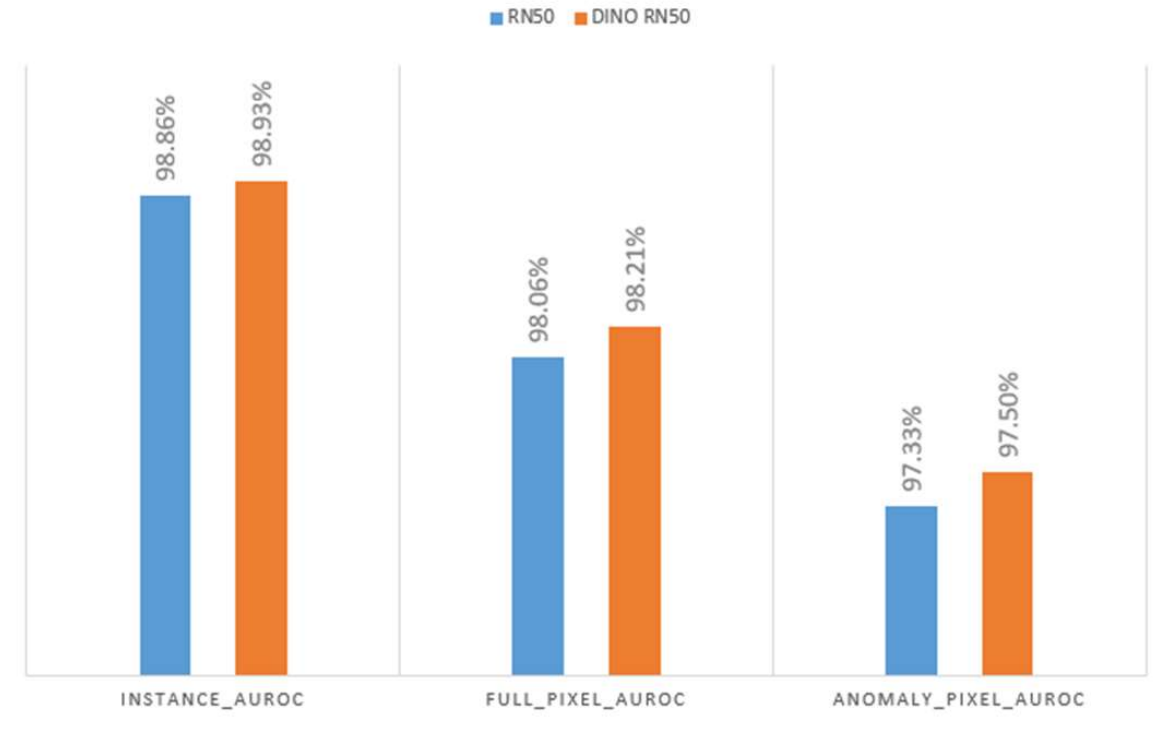
\includegraphics[width=1.0\linewidth]{Chapter_4/dino.png}
	\end{center}
	\caption{Comparison of mean Instance AUROC, Full Pixel AUROC and Anomaly AUROC scores of ResNet50 pre-trained with supervised learning and ResNet50 trained with DINO self-supervised model across all categories.}
	\label{fig:dino_test}
\end{figure}

\section{CNN bi-class classifier selective extraction experiments}
\label{sec:comp_vis}

\subsection{Training the CNN bi-class classifier}
We are going to put together a dataset in order to train a CNN bi-class classifier with the method indicated in the Chapter~\ref{chapter:ch3}. The datasets is assembled with the method displayed in the figure \ref{fig:bi_class_prep}. Industrial class of the dataset contains: 454 classes from ImageNet with the removal of images that contain faces prominently, also it contains multiple industrial datasets that are stated in the figure \ref{fig:bi_class_prep}. It is important to note that, the industrial datasets included in the industrial class of the dataset for the training of CNN bi-class classifier, do not reflect on the final learned features that are used in the PatchCore model during test time. We assemble the non-industrial part of the dataset by using 546 classes from ImageNet dataset and Labeled Faces in Wild dataset.

\begin{figure}[h]
	\begin{center}
		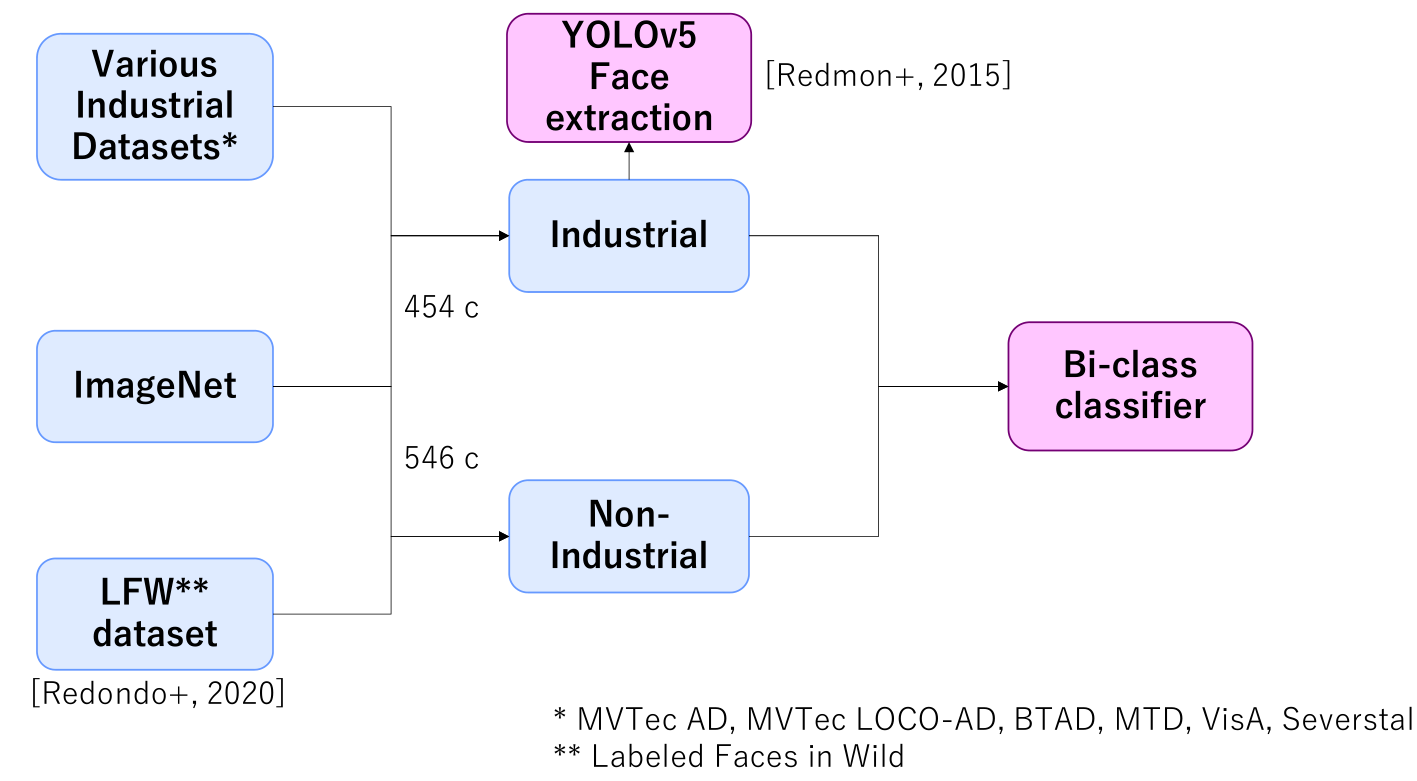
\includegraphics[width=1.0\linewidth]{Chapter_4/bi_class_prep.png}
	\end{center}
	\caption{The detailed explanation of the assembly of the dataset for the training of bi-class classifier.}
	\label{fig:bi_class_prep}
\end{figure}

Using the constructed dataset the extractor model is trained by fine-tuning ImageNet pre-trained ResNet50 model for 25 epochs. The recipe for the fine-tuning is as follows:

\lstset{frame=tb,
  language=Python,
  aboveskip=3mm,
  belowskip=3mm,
  showstringspaces=false,
  columns=flexible,
  basicstyle={\small\ttfamily},
  numbers=none,
  numberstyle=\tiny\color{gray},
  breaklines=true,
  breakatwhitespace=true,
  tabsize=3
}
\begin{lstlisting}
def fine_tune():
	model_ft = models.resnet50(weights='IMAGENET1K_V1')
	num_ftrs = model_ft.fc.in_features
	model_ft.fc = nn.Linear(num_ftrs, len(class_names))
	model_ft = model_ft.to(device)
	criterion = nn.CrossEntropyLoss()
	optimizer_ft = optim.Adam(model_ft.parameters(), lr=0.001)
	exp_lr_scheduler = lr_scheduler.StepLR(optimizer_ft, step_size=7, gamma=0.1)
	model_ft = train_model(model_ft, criterion, optimizer_ft, exp_lr_scheduler, num_epochs=20)
	torch.save(model_ft.state_dict(), 'fine_tuned.pt')
\end{lstlisting}

\subsection{Selective extraction of the dataset for feature learning}
We utilize the trained CNN bi-class classifier to extract an industrial specialized dataset from the YFCC100M dataset. We use the following method to extract the desired samples from the large dataset:


\lstset{frame=tb,
  language=Python,
  aboveskip=3mm,
  belowskip=3mm,
  showstringspaces=false,
  columns=flexible,
  basicstyle={\small\ttfamily},
  numbers=none,
  numberstyle=\tiny\color{gray},
  breaklines=true,
  breakatwhitespace=true,
  tabsize=3
}
\begin{lstlisting}
def predict_image(image_name):
    image = image_loader(image_name)
    with torch.no_grad():
        logits = model.forward(image)
    ps = torch.exp(logits)
    _, predTest = torch.max(ps, 1)
    return predTest[0]

cnt = 0

for (root, dirs, files) in os.walk(address, topdown=True):
    cnt = cnt + 1
    for f in files:
        if f.endswith(".jpg"):
            try:
                t = predict_image(os.path.join(root, f))
            except:
                print(os.path.join(root, f))
            if t == 0:
                os.makedirs(os.path.join(addressDest, str(cnt//1000)), exist_ok=True)
                shutil.copy2(os.path.join(root, f), os.path.join(addressDest, str(cnt//1000), f))
\end{lstlisting}

Here, model refers to bi-class CNN classifier model. After applying this proces to the YFCC100M dataset for a limited amount of time, we receive 2 343 499 industrial samples.

\subsection{Learning features using DINO VitB/16 model}
First batch of feature space comparisons include the state-of-the-art feature extractor ImageNet pre-trained WideResNet50, ImageNet pre-trained VitB/16 and VitB/16 trained with self-supervised learning method DINO. The recipe for training the ImageNet pre-trained WideResNet50 and ImageNet pre-trained VitB/16 is the same as the recipe for ResNet50 stated in the section \ref{sec:dino_tests}. The recipe for the training of VitB/16 on the extracted dataset is as follows (Here, "/po1/rakhimov/extracted" is the extracted dataset.):

\lstset{frame=tb,
  language=bash,
  aboveskip=3mm,
  belowskip=3mm,
  showstringspaces=false,
  columns=flexible,
  basicstyle={\small\ttfamily},
  numbers=none,
  numberstyle=\tiny\color{gray},
  breaklines=true,
  breakatwhitespace=true,
  tabsize=3
}
\begin{lstlisting}
torchrun --nnodes=1 --nproc_per_node=4 main_dino.py --arch vit_base \
--data_path /po1/rakhimov/extracted --output_dir /po1/rakhimov/result \ 
--epochs 100
\end{lstlisting}

It can be understood from the data displayed in the figure \ref{fig:vit_custom_test} that Vision Transformer architecture performs noticably less than CNN architecture. We can draw said conclusion by analysing the performances of ImageNet pre-trained WideResNet50 and VitB/16. Differences in performance are: 6.22\% for Instance AUROC, 2.47\% for Full Pixel AUROC and 2.8\% for Anomaly Pixel AUROC. When it comes to the extracted dataset, although we have efficiency improvement upon VitB/16 trained on ImageNet, overall performance gain over the state-of-the-art feature extractor has not been achieved. Moreover, from this experiment we can conclude that Vision Transformer architecture is unadvisible to use in the further experiments.

\begin{figure}[h]
	\begin{center}
		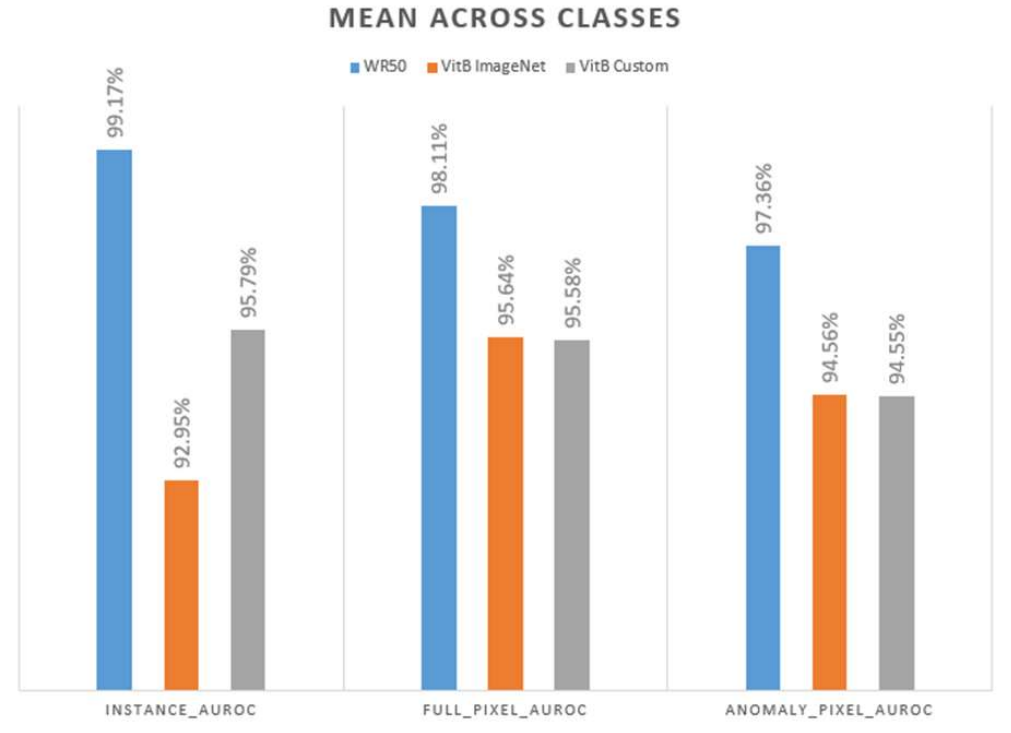
\includegraphics[width=1.0\linewidth]{Chapter_4/vit_custom.png}
	\end{center}
	\caption{Mean scores Instance AUROC, Full Pixel AUROC and Anomaly Pixel AUROC across all categories of MVTechAd dataset}
	\label{fig:vit_custom_test}
\end{figure}

\subsection{Learning features using DINO self-supervised method with the WideResNet50 model}
After the conclusions from the last experiments, we train WideResNet50 using DINO self-supervised method on the extracted dataset. In order to test the efficacy of the selection method, we also train WideResNet50 using the same recipe on 2 343 499 randomly extracted from the YFCC100M dataset. The recipe to train WideResNet50 is as follows:

\lstset{frame=tb,
  language=bash,
  aboveskip=3mm,
  belowskip=3mm,
  showstringspaces=false,
  columns=flexible,
  basicstyle={\small\ttfamily},
  numbers=none,
  numberstyle=\tiny\color{gray},
  breaklines=true,
  breakatwhitespace=true,
  tabsize=3
}
\begin{lstlisting}
torchrun --nproc_per_node=8 main_dino.py --arch wide_resnet50_2 \ 
--optimizer sgd --lr 0.03 --weight_decay 1e-4 \ 
--weight_decay_end 1e-4 --global_crops_scale 0.14 1 \ 
--local_crops_scale 0.05 0.14 --data_path /po1/rakhimov/extracted \ 
--output_dir /po1/rakhimov/result_wd50 --epochs 100
\end{lstlisting}

We also include ResNet50 pre-trained on ImageNet using DINO self-supervised learning method, in order to compare the ImageNet to the extracted dataset when using the same learning method. However, we must also acknowledge that there is difference in the architecture as well. In total, we compare 4 pre-trained feature extractors: ImageNet pre-trained WideResNet50 by supervised classification task, WideResNet50 trained using DINO self-supervised learning model on the selectively extracted dataset, WideResNet50 trained on randomly extracted dataset with DINO model, and ResNet50 trained on ImageNet with DINO model. In the figures \ref{fig:wd_instance}, \ref{fig:wd_anomaly} and \ref{fig:wd_full_pixel} we present Instance AUROC, Anomaly Pixel AUROC and Full Pixel AUROC scores respectively.

Analysing the chart we can notice that in some select few cases the selective extraction reaches, and in some cases, outperforms the sota model. For example, for the Instance AUROC score of bottle, hazelnut and toothbrush classes there is an equal performance between sota feature extractor and the selective extraction method. And for the cases where the selective extraction outperforms the sota model, the examples can be: Full Pixel AUROC scores for carpet, hazelnut, toothbrush, transistor classes. However, we can not conclude that the performance gain is due to the efficacy of the selective extraction method, since there are cases where random extraction outperforms selective extraction. Nevertheless, it is clear that the contents, of the dataset from which features are learned, have a significant importance. Overall, the WideResNet50 pre-trained on ImageNet with supervised classification task stays the best choice for feature extraction.

\begin{figure}[h]
	\begin{center}
		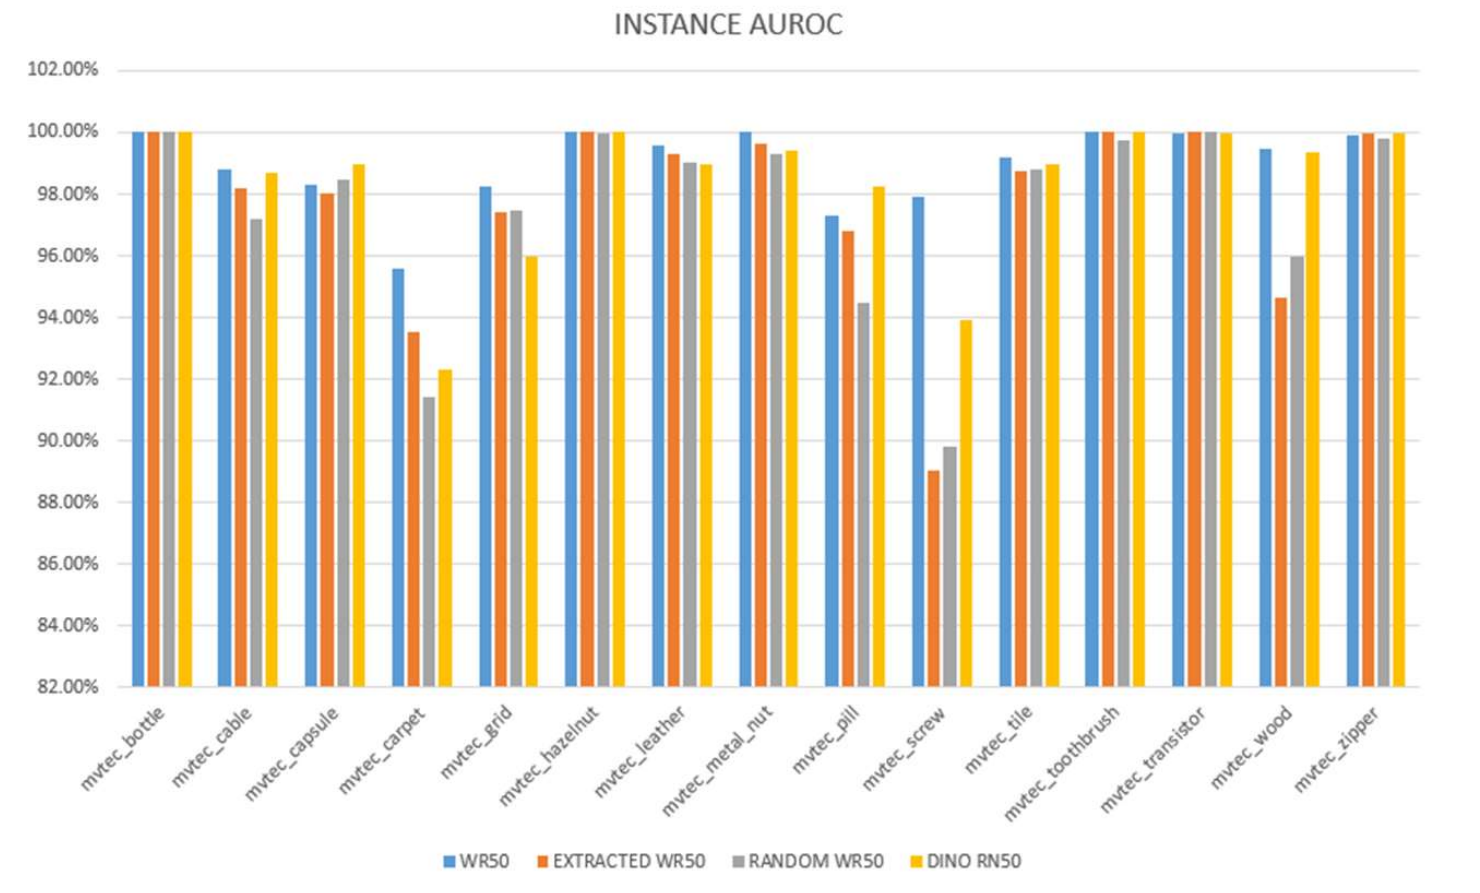
\includegraphics[width=1.0\linewidth]{Chapter_4/wd_instance.png}
	\end{center}
	\caption{Instance AUROC scores across 15 objects in MVTecAD dataset.}
	\label{fig:wd_instance}
\end{figure}

\begin{figure}[h]
	\begin{center}
		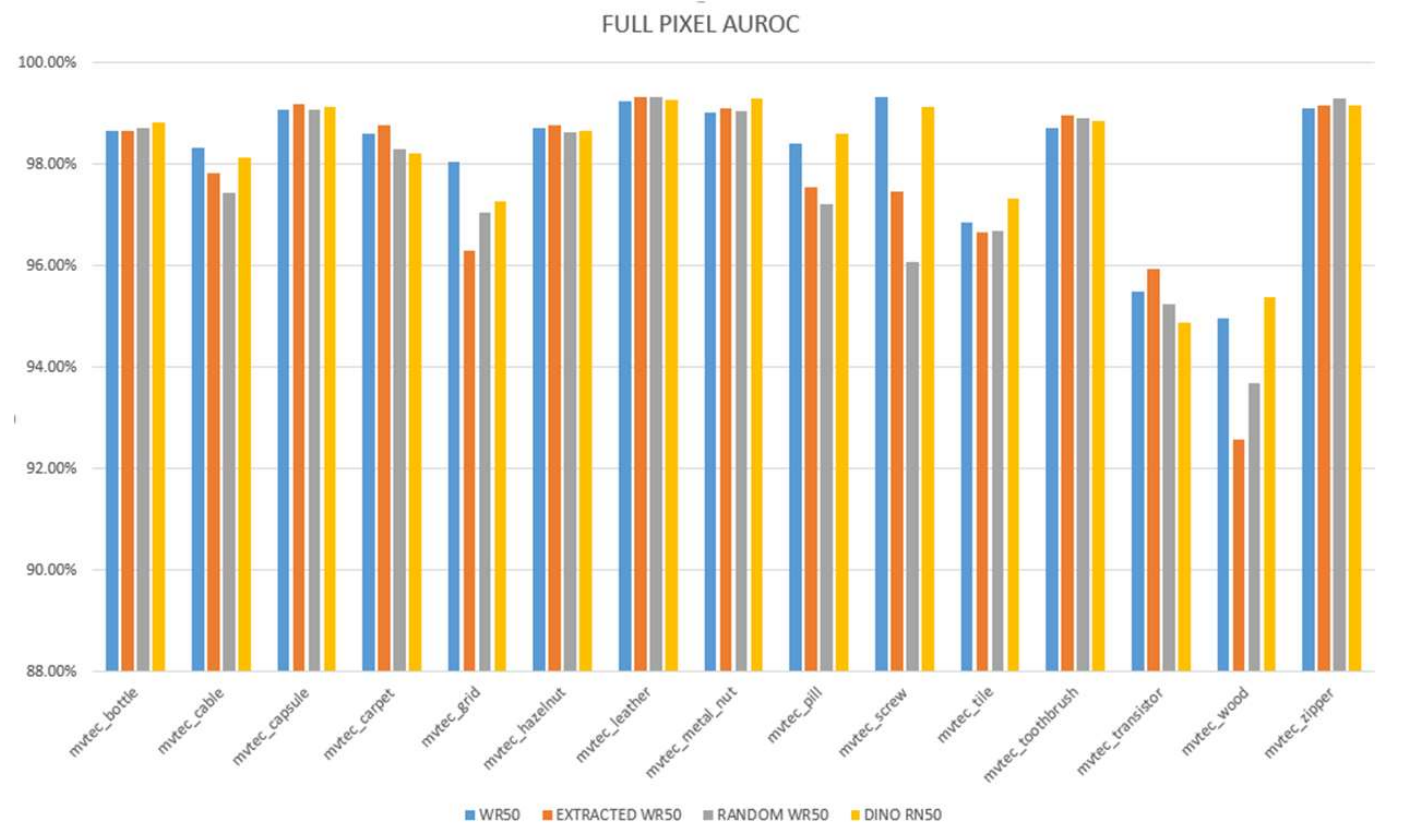
\includegraphics[width=1.0\linewidth]{Chapter_4/wd_full_pixel.png}
	\end{center}
	\caption{Full Pixel AUROC scores across 15 objects in MVTecAD dataset.}
	\label{fig:wd_full_pixel}
\end{figure}

\begin{figure}[h]
	\begin{center}
		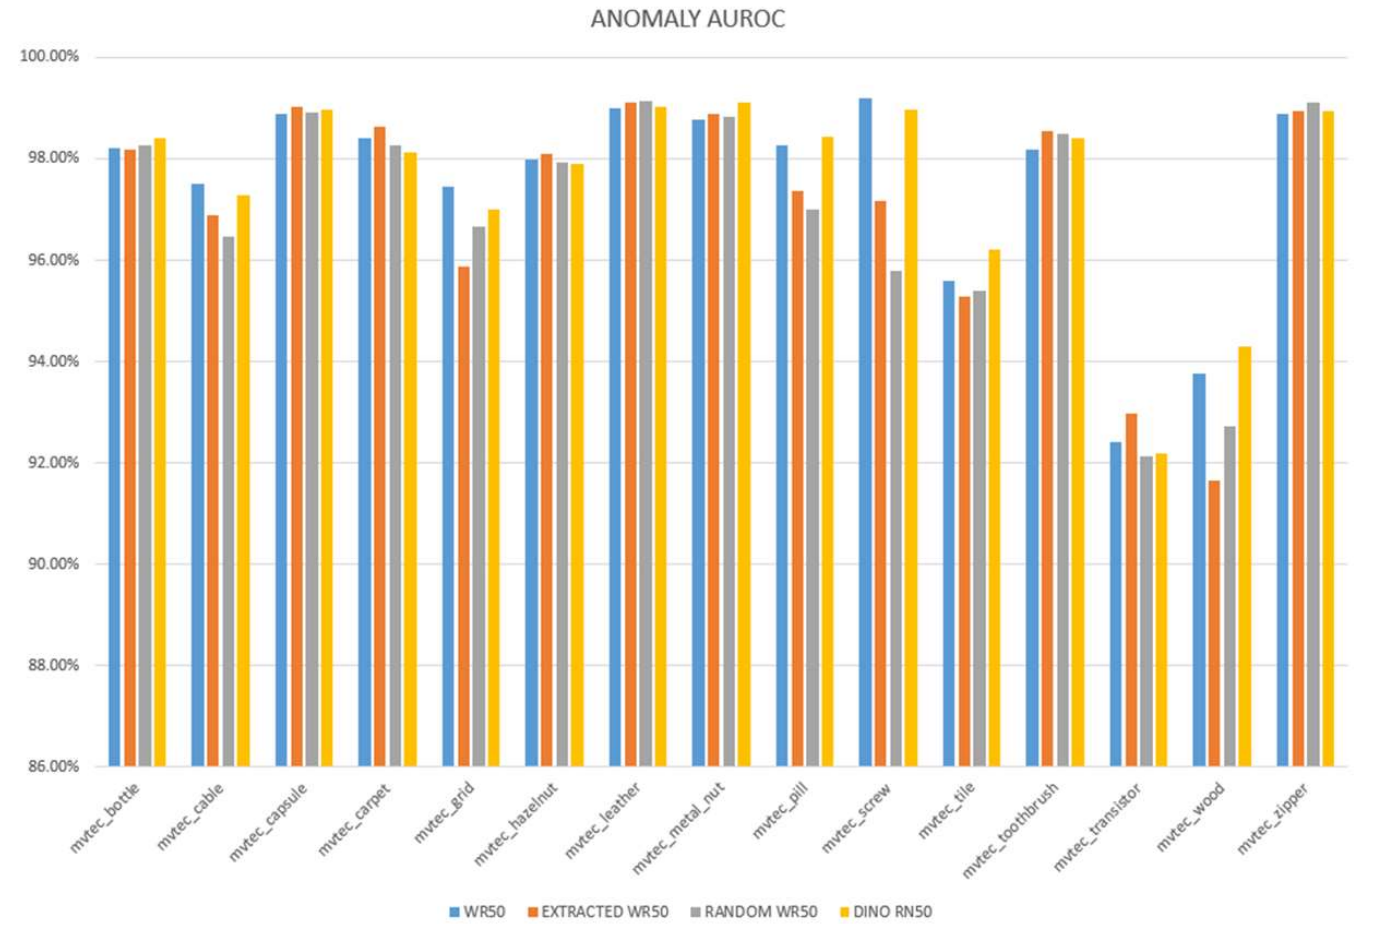
\includegraphics[width=1.0\linewidth]{Chapter_4/wd_anomaly.png}
	\end{center}
	\caption{Anaomaly Pixel AUROC scores across 15 objects in MVTecAD.}
	\label{fig:wd_anomaly}
\end{figure}

\begin{figure}[h]
	\begin{center}
		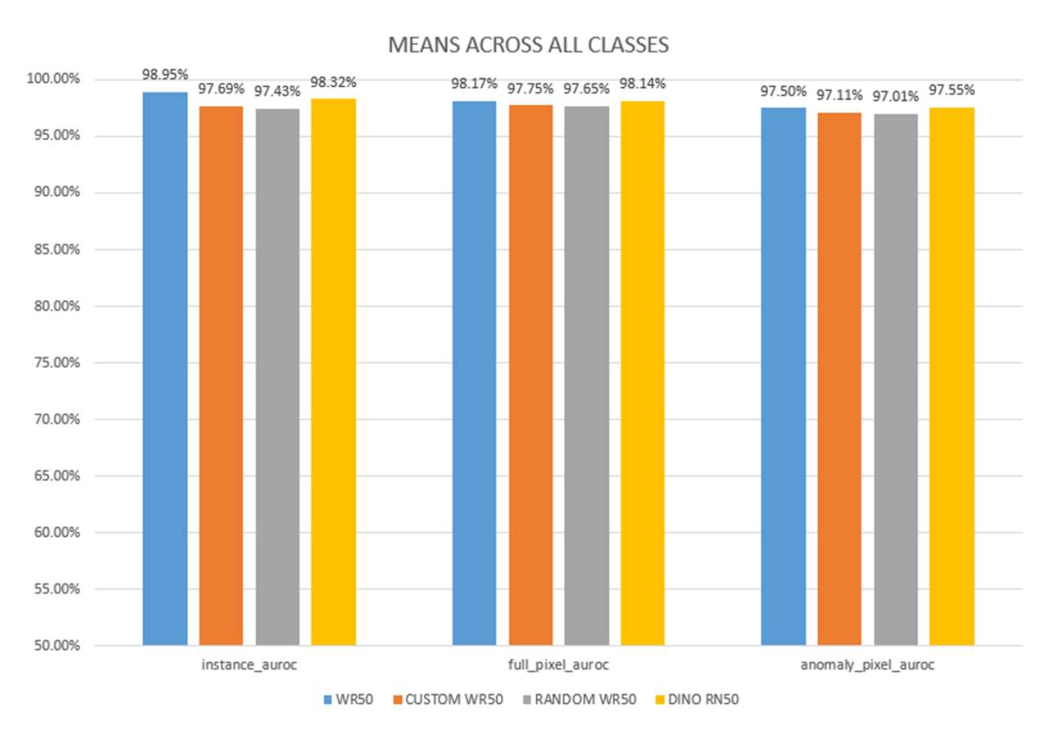
\includegraphics[width=1.0\linewidth]{Chapter_4/wd_mean.png}
	\end{center}
	\caption{Mean scores Instance AUROC, Full Pixel AUROC and Anomaly Pixel AUROC across all categories of MVTechAd dataset}
	\label{fig:wd_mean}
\end{figure}

\section{Selective extraction with LLM and VLM}
Now we will delve into the discussion of the selective extraction method leveraging Large Language Models(LLM) and Vision Language Models(VLM). The LLM of choice for this thesis is GPT-3 and for the VLM, we utilize CLIP model. We follow the pipeline described in the section \ref{sec:llm_and_vlm_extraction}, namely, using GPT-3 model we generate realated suplimentary keywords for 15 classes in the MVTechAD dataset. Further, we generate descriptions using the suplimentary keywords created in the previous step. The total number of keywords and descriptions generates is given in the table \ref{tab:gpt_keywords}.

Next step in the extraction process is to calculate cosine similarities between images and generated descriptions, followed by filtering the samples by the cosine similarity scores that pass the threshold of 0.28. Following code is used to execute this step:

\lstset{frame=tb,
  language=Python,
  aboveskip=3mm,
  belowskip=3mm,
  showstringspaces=false,
  columns=flexible,
  basicstyle={\small\ttfamily},
  numbers=none,
  numberstyle=\tiny\color{gray},
  breaklines=true,
  breakatwhitespace=true,
  tabsize=3
}
\begin{lstlisting}
def clipTest(file, descriptions):
  image = Image.open(file).convert("RGB")
  image_input = torch.tensor(np.stack([preprocess(image)])).cuda()
  desc_tokens = clip.tokenize(descriptions).cuda()
  with torch.no_grad():
      image_features = model.encode_image(image_input).float()
      text_features = model.encode_text(desc_tokens).float()
      image_features /= image_features.norm(dim=-1, keepdim=True)
      text_features /= text_features.norm(dim=-1, keepdim=True)
      similarity = text_features @ image_features.T

      return similarity.max() > 0.28
\end{lstlisting}

\begin{table}[h]
\begin{center}
\begin{tabular}{lll}
\hline 
\textbf{Class} & \textbf{Number of keywords} & \textbf{Number of descriptions} \\
\hline\hline
Bottle & 45 & 40 \\
Cable & 52 & 51 \\
Capsule & 26 & 26 \\
Carpet & 62 & 60 \\
Grid & 43 & 44 \\
Hazelnut & 26 & 29 \\
Leather & 26 & 28 \\
Metal Nut & 47 & 61 \\
Pill & 43 & 27 \\
Screw & 20 & 37 \\
Tile & 68 & 122 \\
Toothbrush & 63 & 107 \\
Transistor & 20 & 29 \\
Wood & 30 & 25 \\
Zipper & 17 & 38 \\
\hline
\end{tabular}
\end{center}
\caption{Numbers of keywords and descriptions generated for each object in the MVTecAD dataset.}
\label{tab:gpt_keywords}
\end{table}

Because of the nature of extaction, specifically the use of keywords, we can easily construct a labeled dataset using base keywords as classes for supervised learning. For feature learning, we fine-tune ImageNet pre-trained WideResNet50 model. We use the same recipe as training the CNN bi-class classifier, with difference being number of output nodes and number of epochs. The model is fine tuned for 100 epochs on 549 197 samples extracted from YFCC100M. As displayed in the figure \ref{fig:llm_clip_mean}, this method does not prove to be effective in generating suitable feature spaces. Nevertheless, it should be mentioned that there is a difference in the number of samples between ImageNet and the extracted dataset. Therefore, it should be considered that with the higher number of samples, there is a possibility of achieving a higher performance.

\begin{figure}[h]
	\begin{center}
		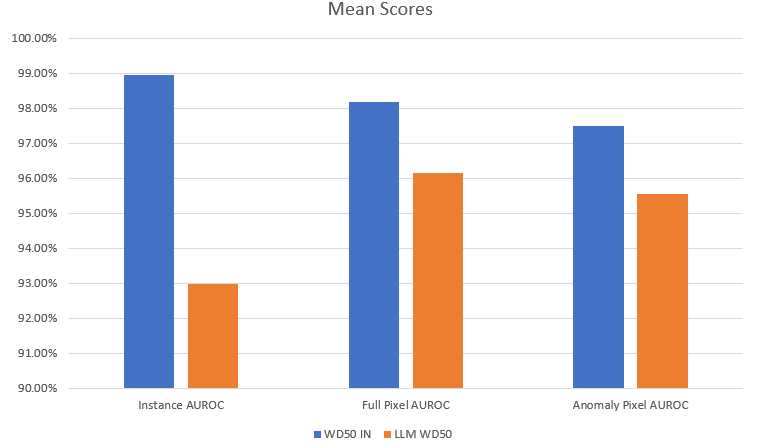
\includegraphics[width=1.0\linewidth]{Chapter_4/llm_clip_mean.png}
	\end{center}
	\caption{Mean scores Instance AUROC, Full Pixel AUROC and Anomaly Pixel AUROC across all categories of MVTechAd dataset}
	\label{fig:llm_clip_mean}
\end{figure}

In this chapter we looked at the empirical analysis on the hypothesis stipulated in the Chapter \ref{chapter:ch3}. In the next chapter, we will draw conclusions based upon the findings discovered througout the research done in this thesis.